\documentclass[a4paper, 12pt]{article}
\usepackage[a4paper, left=30mm, right=30mm, top=30mm, bottom=30mm, marginpar=25mm]{geometry}
\usepackage{indentfirst}
\usepackage{float}
\usepackage{graphicx}
\usepackage{amsmath}
\usepackage{amsfonts}
\usepackage{amssymb}
\usepackage{geometry}
\usepackage{listings}
\usepackage{xcolor}
\usepackage{fancyhdr}
\usepackage{lastpage}
\usepackage[normalem]{ulem} 
\pagestyle{fancy}
\setlength{\headheight}{29.5pt}
\definecolor{codegreen}{rgb}{0,0.6,0}
\definecolor{codegray}{rgb}{0.5,0.5,0.5}
\definecolor{codepurple}{rgb}{0.58,0,0.82}
\definecolor{backcolour}{rgb}{0.95,0.95,0.92}
\lstset{
    backgroundcolor=\color{backcolour},   
    commentstyle=\color{codegreen},
    keywordstyle=\color{blue},
    numberstyle=\tiny\color{codegray},
    stringstyle=\color{codepurple},
    basicstyle=\ttfamily\footnotesize,
    breakatwhitespace=false,         
    breaklines=true,                 
    captionpos=b,                    
    keepspaces=true,                 
    numbers=left,                    
    numbersep=5pt,                  
    showspaces=false,                
    showstringspaces=false,
    showtabs=false,                  
    tabsize=2
}
\usepackage{pgfplots}
\pgfplotsset{compat=1.18}
\usepackage{tikz}
\usepackage{adjustbox}
\usepackage{tikz}
\usepackage{booktabs}
\usepackage{amsmath,amssymb}
\usepackage{tikz}
\usepackage{caption}
\usepackage{algorithm}
\usepackage{algpseudocode}
\usepackage{enumitem}
\usepackage{hyperref}
\renewcommand{\contentsname}{Índice}

\renewcommand*{\maketitle}{
\thispagestyle{plain}
\begin{center}
    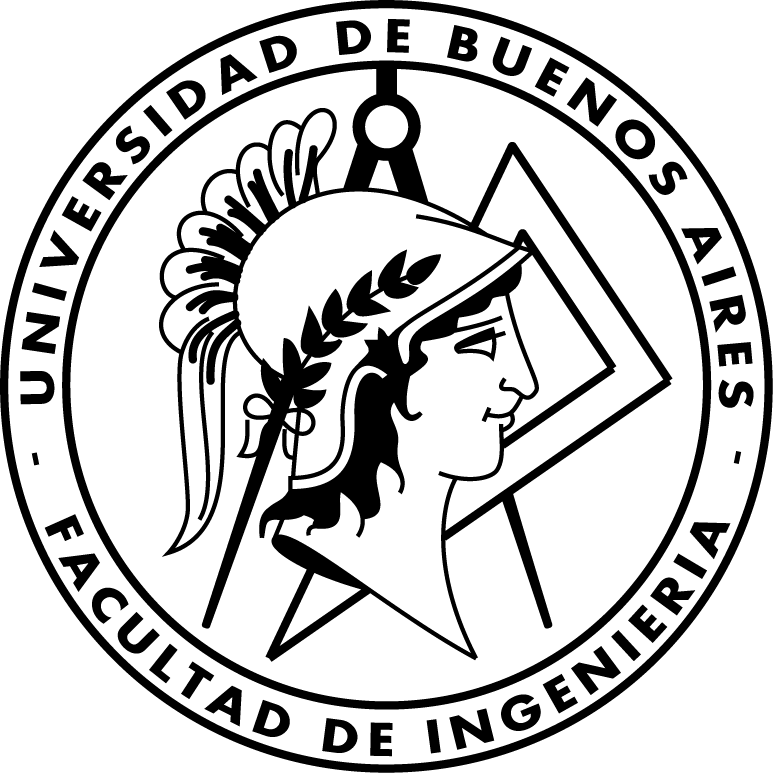
\includegraphics[width=7cm]{Logo-fiuba.png} 
    \\[1cm]
    \textsc{\Large Teoría de Algoritmos}\\           
    \textsc{\small Curso Echevarria}\\[0.4cm]    
    { \huge \bfseries Trabajo Práctico 1 }\\[0.3cm]      
    \rule{\textwidth}{0.4pt} \\[0.2cm] 
    {\large \today  \\[0.5cm]}                          
    \begin{minipage}{0.6\textwidth}
    \begin{flushleft}
        \large{
        \begin{itemize}
            \item Juan Claros - 111254
            \item Yoel Gaston Arlia - 111520
            \item Guido Cuppari - 111172
            \item Josue Daniel Mamani - 111514
        \end{itemize}
        }
    \end{flushleft}
\end{minipage}

\end{center}
}

\title{x}

\begin{document}

\maketitle

\newpage

\tableofcontents

\newpage
\section{{\uline{\textbf{\textit{Problema 1}}}}}
\subsection{Enunciado y Supuestos}
\begin{itemize}
    \subsubsection{Enunciado}
    \item 
    Cualquier cadena puede ser descompuesta en secuencias de palíndromos. Por ejemplo, la 
    cadena ARACALACANA se puede descomponer de las siguientes formas: 
    ARA CALAC ANA \\
    ARA C ALA C ANA \\
    A R A CALAC A N A \\
    etc. \\
    Desarrollar un algoritmo de programación dinámica que encuentre el menor número de 
    palíndromos que forman una cadena dada. Por ejemplo, para ARACALACANA debería 
    devolver 3.
    \subsubsection{Supuestos}
    \item Se supone que el algoritmo recibe una cadena (string), con una frase, y el algoritmo buscara la mínima cantidad de palíndromos posibles que forma la cadena dada por parámetro, mediante programación dinámica.
    \item La frase, si tiene espacios o caracteres especiales, van a ser tratados como letras, ejemplo A!NEUQUEN!A, va a devolver 1, ya que se es indiferente con los caracteres y letras.
    \end{itemize}
\subsection{Diseño}
\begin{itemize}
\item La ecuación de recurrencia a la que se llego es: \(opt[i] = 1\) si \(palabra[i:]\) es palíndromo y \(opt[i] = min(opt[j+1] + 1)\) para todo j tal que \(palabra[i:j+1]\) es palíndromo.

\item Subestructura óptima: La solución óptima para el prefijo \(palabra[0:i]\) depende de las soluciones óptimas de los sufijos \(palabra[j+1:]\), que son subproblemas del problema original.

Subproblemas superpuestos: Evaluar si una subcadena es palíndromo se repite muchas veces. Por eso se usa una tabla booleana \(\texttt{es\_palindromo}[i][j]\) para memorizar los resultados.

\item Se usa memoization en 2 estructuras de datos, para guardar en un arreglo de enteros (todos infinitos positivos de base) \(opt[i]\) el mínimo numero de palíndromos para \(palabra[i:]\). Y para guardar en una matriz booleana (con todas las posiciones false de base) de n x n \(\texttt{es\_palindromo}[i][j]\) si \(palabra[i:j+1]\) es un palíndromo.

\item Las estructuras de datos utilizadas para esta resolución son una lista de enteros, y una matriz de booleanos, siendo opt la lista y es\_palíndromo la matriz.

\newpage
\subsection{Pseudocodigo}
	\begin{lstlisting}[frame=single]
FUNCION min_palindromos(palabra):
    n = largo(palabra)
    
    optimo = [float('infinito')] * (n + 1)
    opt[n] = 0

    es_palindromo = [[False] * n for _ in range(n)]

    Para i desde n - 1 hasta 0 con paso -1 hacer
        Para j desde i hasta n - 1 hacer
            Si palabra[i] = palabra[j] y (j - i <= 1 o es_palindromo[i + 1][j - 1]) entonces
                es_palindromo[i][j] <- Verdadero
            FinSi
        FinPara
    FinPara

    Para i desde n - 1 hasta 0 con paso -1 hacer
        Para j desde i hasta n - 1 hacer
            Si es_palindromo[i][j] entonces
                opt[i] <- minimo entre opt[i] y (1 + opt[j + 1])
            FinSi
        FinPara
    FinPara


    DEVOLVER opt[0]

cadena = "ALLAERRESAGASRADAR"
print(min_palindromos(cadena))
	\end{lstlisting}

\end{itemize}

\newpage
\subsection{Análisis de Complejidad}
\begin{itemize}
    \item Los puntos clave para analizar la complejidad de este algoritmo son los 2 for anidados que hay tanto para el procesamiento de los palíndromos que se ejecuta para cada par i,j en:
    
	\begin{lstlisting}[frame=single]
    for i in range(n - 1, -1, -1):
        for j in range(i, n):
            if palabra[i] == palabra[j] and (j - i <= 1 or es_palindromo[i + 1][j - 1]):
                es_palindromo[i][j] = True
	\end{lstlisting}

    Y para la construcción de la tabla booleana opt[i][j] que también revisa cada subcadena \(palabra[i:j+1]\), y si la misma es palíndromo realiza una operación constante en: 
    \begin{lstlisting}[frame=single]
    for i in range(n - 1, -1, -1):
        for j in range(i, n):
            if es_palindromo[i][j]:
                opt[i] = min(opt[i], 1 + opt[j + 1])
	\end{lstlisting}

    Por lo tanto, en ambos for anidados, el peor caso implica una doble iteración sobre n, por ende la complejidad temporal total del algoritmo es de \(O(N^2)\), siendo N el largo de la cadena. 

\end{itemize}

\newpage
\subsection{Seguimiento}
\begin{itemize}
\item Vamos a hacer el seguimiento para el caso de la cadena "ARACALACANA": lo primero que hace el algoritmo es obtener el largo de la cadena recibida mediante len(), normalizar todo a mayúsculas y procede a generar las 2 estructuras utilizadas, la lista de enteros y la matriz de booleanos, para luego llegar a la primer parte importante, el preprocesamiento de los , donde se marca como True toda subcadena de \(palabra[i:j+1]\) que sea un palíndromo.

    \subitem $n = \text{largo}(\text{palabra}) = 11$
        \subitem \texttt{opt = [inf, inf, ..., inf, 0]} (longitud 12)
        \subitem \texttt{es\_palindromo[i][j] = False} para toda $i, j$

\item Para ver si un substring es palíndromo o no, se utilizan 3 factores, si palabra[i] = palabra[j] (la palabra empieza y termina con la misma letra) y si \(j - i  <= 1\) (es de 1 o 2 caracteres) o \(\texttt{es\_palindromo}[i+1][j-1]\) = True. Entonces empieza desde i = 10 y siempre lo primero que llena en cada i es la diagonal, que es trivialmente un palíndromo, al ser un solo carácter, pero empieza llenando la matriz desde el final.

\item La primer posición analizada es [10][10], siendo la cadena "A", que es un caso trivial, cumpliendo la condición y llenando la tabla en esa posición con True, luego sigue [9][9], que ocurre lo mismo que en el caso anterior, siendo simplemente el carácter "N", [9][10] no cumple la condición, ya que no empieza y termina con la misma letra, quedándose en False..., saltamos al ejemplo del siguiente palíndromo no trivial, que es [8][10] la cadena "ANA" cumple que empieza y termina con la misma letra, no tiene menos de 2 caracteres, pero \(\texttt{es\_palindromo}[i+1][j-1]\) que en este caso es [9][9] es True, entonces rellena True dándola como palíndromo.

\item Para el final de las iteraciones el algoritmo rellena la tabla ubicando True en todos los palíndromos que encuentra.

\begin{figure}[H]
    \centering
    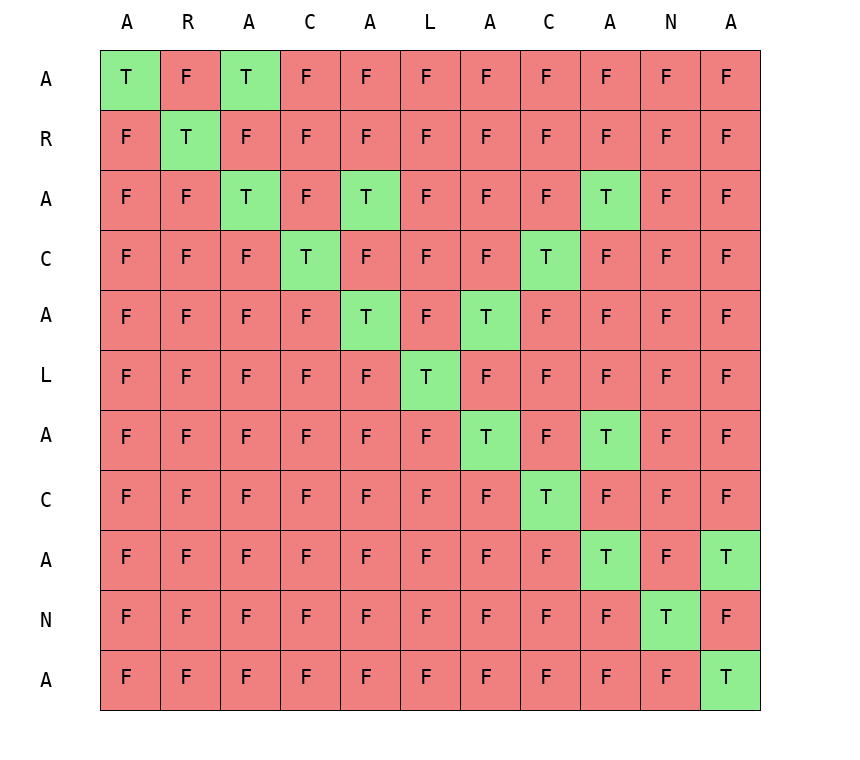
\includegraphics[width=\textwidth]{matriz_palindromos_ARACALACANA.png}
    \caption{Representación de la matriz de palíndromos.}
    \label{fig:matriz_palindromos_ARACALACANA.png}
\end{figure}


\item Una vez rellenada la tabla, pasa a la construcción de opt[i] buscando la mínima cantidad de palíndromos de la palabra, donde opt[n] = 0, siendo el caso base la string vacía, luego empieza la iteración desde i = 10 hasta 0.

\item Entonces empieza con [10][10], le pregunta a la tabla si es palíndromo, en este caso lo es, por ende opt[i] es igual al mínimo entre si mismo, que de base es infinito, y 1 + opt[j+1], que en este caso es 1 + opt[11] (que es 0), entonces opt[10] = 1. Sigue con i = 9, j = 9, se le pregunta si la [9][9] es True, lo cual es correcto, entonces se usa la ecuación siendo opt[9] = min(opt[9], 1 + opt[10], que termina siendo opt[9] = min(infinito, 2), opt[9] = 2, y así sigue con toda la tabla para finalmente encontrar el optimo que es 3.

\end{itemize}

\newpage
\subsection{Casos de prueba y mediciones}
\begin{tabular}{@{}lcc@{}}
\toprule
Entrada & Cantidad de palíndromos & Tiempo (ms) \\
\midrule
radaroso              & 2  & 0.077725 \\
123456789             & 9  & 0.077863 \\
amor a roma           & 1  & 0.108240 \\
JuanJoseGuidoYoel     & 15 & 0.162336 \\
ppppppppppppppppppp      & 1  & 0.439882 \\
anilinareconocersalas & 3  & 0.304222 \\
\bottomrule
\end{tabular}
\subsection{Resultados}
\section*{Tiempo de ejecución vs longitud de la cadena (N)}

\begin{center}
\begin{tikzpicture}
\begin{axis}[
    width=14cm,
    height=9cm,
    xlabel={Longitud de la cadena (N)},
    ylabel={Tiempo de ejecución (ms)},
    grid=major,
    enlargelimits=0.1,
    title={Relación entre longitud N y tiempo de ejecución},
    ymin=0, ymax=0.5
]

% Coordenadas con nombres como etiquetas
\addplot[
    color=blue,
    mark=*,
    thick
] coordinates {
    (8,0.077725)
    (9,0.077863)
    (10,0.108240)
    (18,0.162336)
    (20,0.439882)
    (21,0.304222)
};

% Etiquetas manuales
\node at (axis cs:8,0.077725) [above left, font=\tiny] {radaroso};
\node at (axis cs:9,0.077863) [above right, font=\tiny] {123456789};
\node at (axis cs:10,0.108240) [above left, font=\tiny] {amor a roma};
\node at (axis cs:18,0.162336) [above right, font=\tiny] {JuanJoseGuidoYoel};
\node at (axis cs:20,0.439882) [below, font=\tiny] {pppppppppppppppppppp};
\node at (axis cs:21,0.304222) [above right, font=\tiny] {anilinareconocersalas};

\end{axis}
\end{tikzpicture}
\end{center}
\section*{Curva de \(N^2\)}

\begin{center}
\begin{tikzpicture}
\begin{axis}[
    width=12cm,
    height=8cm,
    xlabel={N},
    ylabel={\(N^2\)},
    grid=major,
    domain=0:25,
    samples=100,
    title={Gráfico de \(N^2\)},
    thick
]
\addplot[
    color=blue,
    no markers
]
{x^2};
\end{axis}
\end{tikzpicture}
\end{center}

\subsection{Conclusiones}
\begin{itemize}
    \item Se ve que los sets cumplen con la complejidad prevista, exceptuando el caso de las p, donde se deja ver que las operaciones descartadas por ser menores a $N^2$ afectan a la complejidad, exceptuando este caso, se ve que a medida que aumenta el largo, el tiempo sube exponencialmente, cumpliendo lo previsto.
\end{itemize}
\subsection{Generación de sets}
\begin{itemize}
    \item Los sets fueron generados arbitrariamente, para poder probar casos como distinción entre minúscula y mayúscula, espacios, ningún palíndromo, palindromos encadenados, y una cadena de un solo carácter.
\end{itemize}

\newpage
\section{{\uline{\textbf{\textit{Problema 2}}}}}
\subsection{Enunciado y Supuestos}
\begin{itemize}
    \subsubsection{Enunciado}
    \item 
    Concesiones Argentina 2000 SRL tiene la concesión de los espacios publicitarios en las paradas de colectivos de un municipio. Son en total 200 paradas y tiene ofertas de distintos productos para el próximo mes: 
     \item Cliente A ofrece USD 50000 por ocupar 30 paradas 
     \item Cliente B ofrece USD 100000 por ocupar 80 paradas o \item USD 120000 por 120 paradas (sólo una de ambas opciones) 
     \item Cliente C ofrece USD 100000 por ocupar 75 paradas 
     \item Cliente D ofrece USD 80000 por ocupar 50 paradas 
     \item Cliente E ofrece USD 5000 por ocupar 2 paradas 
     \item Cliente F ofrece USD 40000 por ocupar 20 paradas 
     \item Cliente G ofrece USD 90000 por ocupar 100 paradas 
    \item Por ser competidores directos, no se puede hacer publicidad simultáneamente de los clientes A y D. Se desea determinar a qué clientes se concesionará la publicidad de las paradas para maximizar el beneficio total. 
    \subsubsection{Supuestos}
Para el planteamiento del modelo se asumen las siguientes premisas:
    \item El entorno es determinístico; los datos de entrada se conocen exactamente sin error.
    \item Las relaciones entre variables son lineales, por lo que cualquier término no lineal se desprecia.
    \item Los recursos y demandas involucrados están completamente definidos y son medibles, permitiendo una modelación precisa.
    \item Se asume que los costos y beneficios pueden expresarse como funciones lineales de las variables de decisión.
    \item No se consideran incertidumbres, variaciones estocásticas ni fenómenos externos que puedan afectar la solución.
\end{itemize}
\vspace{1.5cm}
\subsection{Variables del Modelo}
En el modelo se definen las siguientes variables:
\subsubsection{Variables}
    las variables para resolver el problema son las siguientes:
\begin{itemize}
    \item a = incluir cliente A (variable binaria)
    \item $b_1$ = incluir cliente B de 80 paradas (variable binaria)
    \item $b_2$ = incluir cliente B de 120 paradas (variable binaria)
    \item c = incluir cliente C (variable binaria)
    \item d = incluir cliente D (variable binaria)
    \item e = incluir cliente e (variable binaria)
    \item f = incluir cliente f (variable binaria)
    \item g = incluir cliente G (variable binaria)
\end{itemize}

\subsection{Modelo de programación lineal}
    La función objetivo a maximizar es la siguiente:
\begin{align*}
    z &= 50000a + 100000b_1 + 120000b_2 + 100000c + 80000d + 5000e + 40000f + 90000g \\
    \max(z)
\end{align*}

Restricciones del modelo:
\begin{align*}
    30a + 80b_1 + 120b_2 + 75c + 50d + 2e + 20f + 100g &\leq 200 \\
    b_1 + b_2 &\leq 1 \\
    a + d &\leq 1
\end{align*}
\begin{itemize}
    \item La primera ecuación nos indica el total de paradas de se concesionaria a los clientes para la publicidad no supere las 200 paradas disponibles.
    \item La segunda ecuación nos indica que de las ambas opciones que tiene el cliente B solo pueda ser 1 y no las 2.
    \item La tercera ecuación nos indica que no se puede hacer publicidad simultáneamente de los cliente A y D.
    
\end{itemize}

\subsection{Solución}
    Para resolver el modelo se desarrollo un programa utilizando Python y PuLP, el cual es el siguiente:
    \begin{figure}[H] 
		\centering
		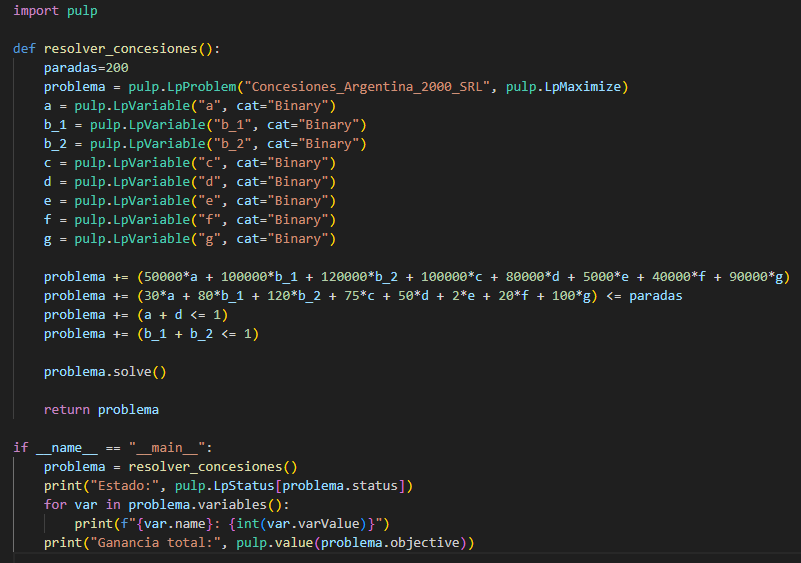
\includegraphics[width=\textwidth]{modelo.png}
	\end{figure}

    Como resultado dio que para maximizar la ganancia tendríamos que escoger a los clientes A, B\_1(la opción de 80 paradas), C y E.

\subsection{Informe}
    La solución del modelo de programación lineal nos propone que para determinar a qué clientes se concesionará la publicidad de las paradas para maximizar el beneficio total son las siguientes:
\begin{itemize}
    \item Cliente A ofrece USD 50000 por ocupar 30 paradas 
    \item Cliente B ofrece USD 100000 por ocupar 80 paradas
    \item Cliente C ofrece USD 100000 por ocupar 75 paradas 
    \item Cliente E ofrece USD 5000 por ocupar 2 paradas 
\end{itemize}
    Con estos resultados nos queda una ganancia de USD 255000 y la cantidad de paradas utilizadas para la publicidad son de 187, la cantidad de paradas no llega al limite pero tampoco se puede utilizar para darles publicidad a otros clientes porque las paradas requeridas por los otros clientes es mayor a la disponible.

    \newpage
\section{{\uline{\textbf{\textit{Problema 3}}}}}
\subsection{Enunciado y Supuestos}
\begin{itemize}
    \subsubsection{Enunciado}
    \item Estamos construyendo una red WAN con n antenas y queremos que tenga un buen nivel de tolerancia a fallas. Dada una antena, su conjunto de backup de tamaño k es el conjunto de k antenas que se encuentran a una distancia menor a D. Queremos evitar que una antena pertenezca al conjunto de backup de más de b antenas, precisamente para evitar que un fallo pueda afectar a una porción importante de la red. Suponer que conocemos los valores D, b y k, y que tenemos una matriz d[1..n, 1..n] con las distancias entre antenas, de forma tal que d[i,j] es la distancia entre la antena i y la j. 
    
    Plantear un algoritmo de complejidad polinomial que encuentre el conjunto de backup de tamaño k de cada una de las n antenas, de forma tal que ninguna aparezca en más de b conjuntos de backup, o bien, que indique que no existe una solución posible. Debe apoyarse en el algoritmo estándar de Ford-Fulkerson, la variante escalada o la de Edmonds-Karp.
    \subsubsection{Supuestos}
    \item
    \begin{enumerate}[label=\arabic*.]
        \item \textbf{Datos de Entrada:} Se dispone de una matriz de distancias \(d[1 \dots n,\,1 \dots n]\) donde \(d[i,j]\) es la distancia entre la antena \(i\) y la \(j\). Se asume que dicha matriz está completa, es decir, se conocen todas las distancias relevantes para la red.
        \item \textbf{Distancia Umbral:} Solo se consideran como candidatos backup aquellas antenas que se encuentran a una distancia menor a \(D\) respecto a la antena en cuestión.
        \item \textbf{Tamaño del Conjunto de Backup:} Para cada antena se debe seleccionar exactamente un conjunto de backup de tamaño \(k\).
        \item \textbf{Restricción de Uso:} Una antena puede formar parte del backup de, a lo sumo, \(b\) otras antenas. Esto previene la sobrecarga y, en caso de fallo, evita que el problema se propague a una parte importante de la red.
        \item \textbf{No Auto-backup:} Se asume que una antena no puede ser backup de sí misma (es decir, no existen bucles desde un nodo a sí mismo en la red de flujo).
        \item \textbf{Linealidad y Exactitud:} Se supone que los datos son exactos y que las relaciones (por ejemplo, “estar a menos de \(D\)”) se definen de forma lineal y determinística.
    \end{enumerate}
    \end{itemize}

    \subsection{Diseño del Algoritmo}
El algoritmo se basa en la modelación del problema vía una red de flujo, y se resuelve mediante un algoritmo clásico (por ejemplo, Ford-Fulkerson, su variante escalada o Edmonds-Karp). A continuación se describen los pasos para adaptar los datos de entrada a una red de flujo y cómo interpretar la salida.

\subsection{Adaptación a una Red de Flujo y Significado de la Salida}
\paragraph{Construcción de la Red de Flujo:}
Se genera un grafo dirigido que transformará el problema de asignación de backups en un problema de flujo:
\begin{enumerate}[label=\alph*.]
    \item \textbf{Nodos:}
    \begin{itemize}
        \item Se crea un nodo fuente \(S\) y un nodo sumidero \(T\).
        \item Se representan las antenas en dos copias: la parte izquierda (o de origen) y la parte derecha (o de destino). La copia de la izquierda representa a cada antena que debe elegir \(k\) backups; la copia de la derecha representa a cada antena como potencial backup, con su límite de participación.
    \end{itemize}
    \item \textbf{Arcos desde la Fuente:}  
    Se crea un arco desde \(S\) a cada antena (en la copia izquierda) con capacidad \(k\). Esto asegura que cada antena debe “enviar” \(k\) unidades de flujo, interpretadas como la cantidad de backups necesarios.
    
    \item \textbf{Arcos Intermedios:}  
    Se conecta una antena \(i\) (de la copia izquierda) con una antena \(j\) (en la copia derecha) mediante un arco de capacidad 1 si y sólo si \(d[i,j] < D\). Esta condición garantiza que únicamente se consideren antenas \emph{cercanas} (según el umbral \(D\)).
    
    \item \textbf{Arcos al Sumidero:}  
    Cada antena \(j\) (de la copia derecha) se conecta con el sumidero \(T\) mediante un arco de capacidad \(b\). Esto impone que ninguna antena sea asignada como backup a más de \(b\) antenas.
\end{enumerate}

\paragraph{Interpretación de la Salida:}
Una vez construida la red, se ejecuta el algoritmo de flujo, Edmonds-Karp. Si el flujo máximo encontrado es exactamente \(n \cdot k\) (ya que cada una de las \(n\) antenas debe enviar \(k\) unidades de flujo), entonces:
\begin{itemize}
    \item La solución asigna, para cada antena \(i\), un conjunto de \(\{ j \mid \text{flujo en el arco } (i, j) = 1 \}\) de tamaño \(k\).
    \item Cada antena \(j\) aparecerá en el conjunto de backup de al menos 0 y como máximo \(b\) antenas, dado el límite impuesto en el arco de \(j\) a \(T\).
\end{itemize}
Si el flujo máximo es menor que \(n \cdot k\), se concluye que no es posible asignar respaldos cumpliendo todas las restricciones.

\paragraph{Diagrama de la Red de Flujo:}
A continuación se muestra un diagrama esquemático de la modelación:

\begin{center}
\begin{tikzpicture}
    % Nodos fuente y sumidero
    \node[draw, circle] (S) at (0,0) {\(S\)};
    \node[draw, circle] (T) at (8,0) {\(T\)};
    
    % Nodos del lado izquierdo (origen)
    \node[draw, rectangle] (A1) at (2,-1) {\(1\)};
    \node[draw, rectangle] (A2) at (2,-2) {\(2\)};
    \node[draw, rectangle] (A3) at (2,-3) {\(\vdots\)};
    
    % Nodos del lado derecho (destino)
    \node[draw, rectangle] (B1) at (6,-1) {\(1\)};
    \node[draw, rectangle] (B2) at (6,-2) {\(2\)};
    \node[draw, rectangle] (B3) at (6,-3) {\(\vdots\)};
    
    % Arcos de S a nodos de la izquierda (capacidad = k)
    \draw[->] (S) -- (A1) node[midway, above] {\(k\)};
    \draw[->] (S) -- (A2) node[midway, above] {\(k\)};
    \draw[->] (S) -- (A3) node[midway, above] {\(k\)};
    
    % Arcos entre nodos izquierdos y derechos
    \draw[->] (A1) -- (B2) node[midway, above] {\(1\)};
    \draw[->] (A1) -- (B3) node[midway, above] {\(1\)};
    \draw[->] (A2) -- (B1) node[midway, above] {\(1\)};
    \draw[->] (A2) -- (B3) node[midway, above] {\(1\)};
    
    % Arcos de nodos de la derecha al sumidero (capacidad = b)
    \draw[->] (B1) -- (T) node[midway, above] {\(b\)};
    \draw[->] (B2) -- (T) node[midway, above] {\(b\)};
    \draw[->] (B3) -- (T) node[midway, above] {\(b\)};
\end{tikzpicture}

\captionof{figure}{Modelo de Red de Flujo para la Asignación de Backups}
\end{center}

\subsection{Pseudocódigo y Estructuras de Datos Utilizadas}
A continuación se presenta un pseudocódigo que resume el proceso completo:


\begin{lstlisting}[frame=single, caption={Pseudocódigo para construir el grafo y asignar respaldo}]
FUNCION Construir_Grafo(distancias, D, b, k):
    n <-- longitud(distancias)
    Crear grafo dirigido G vacio
    fuente  <-- "S"
    sumidero <-- "T"
    
    Agregar nodo fuente a G
    Agregar nodo sumidero a G
    
    Para i desde 0 hasta n-1 hacer:
        entrada <-- "in_" concatenado con i
        salida  <-- "out_" concatenado con i
        Agregar nodo "entrada" a G
        Agregar nodo "salida" a G
        Agregar arco (fuente, entrada) con capacidad k a G
        Agregar arco (salida, sumidero) con capacidad b a G
    
    Para i desde 0 hasta n-1 hacer:
        Para j desde 0 hasta n-1 hacer:
            Si (i ! = j) y (distancias[i][j] < D) entonces:
                Agregar arco ("in_" concatenado con i, "out_" concatenado con j)
                con capacidad 1 a G  
    Retornar G

FUNCION Asignar_Respaldo(distancias, D, b, k):
    G <-- Construir_Grafo(distancias, D, b, k)
    (flujo_total, flujo) <-- CalcularFlujoMaximo(G, "S", "T")
    n <-- longitud(distancias)
    
    Si flujo_total < n * k entonces:
        Retornar "No existe solucion"
    
    resultado <-- arreglo de n listas vacias
    
    Para i desde 0 hasta n-1 hacer:
        entrada <-- "in_" concatenado con i
        Para j desde 0 hasta n-1 hacer:
            Si (i ! = j) y (distancias[i][j] < D) entonces:
                salida <-- "out_" concatenado con j
                Si flujo[entrada][salida] = 1 entonces:
                    Agregar j a resultado[i]
    Imprimir resultado
    Retornar resultado
\end{lstlisting}

\paragraph{Estructuras de Datos:}
\begin{itemize}
    \item \textbf{Grafo \(G\):} Representado mediante listas de adyacencia (o matriz de adyacencia) donde cada arco almacena su capacidad y flujo actual.
    \item \textbf{Nodos:} Cada antena se divide en dos nodos (\(u_i\) y \(v_i\)) para representar su rol como emisor y receptor en la red.
    \item \textbf{Cola:} En la implementación de Edmonds-Karp se utiliza una cola para el recorrido en anchura (BFS) en búsqueda de caminos aumentantes.
    \item \textbf{Arcos:} Cada arco se representa como una estructura o tupla con información sobre el nodo origen, nodo destino, capacidad máxima y flujo actual.
\end{itemize}
\subsection{Ejemplo de Seguimiento con Datos Reducidos}

Consideremos el siguiente set reducido de datos:

\begin{itemize}
    \item Número de antenas: \( n = 3 \).
    \item Valor de umbral de distancia: \( D = 2 \).
    \item Tamaño de respaldo requerido: \( k = 1 \) (cada antena necesita un backup).
    \item Límite de apariciones como backup: \( b = 1 \) (cada antena puede servir como backup para, a lo sumo, una otra antena).
    \item Matriz de distancias:
      

\[
      \begin{pmatrix}
      0 & 1 & 1 \\
      1 & 0 & 1 \\
      1 & 1 & 0 \\
      \end{pmatrix}
      \]


\end{itemize}

Dado que \(d[i][j] = 1 < D\) para \(i \neq j\), cada antena \(i\) podrá conectarse a las otras dos antenas \(j\).

Sin embargo, considerando las restricciones de capacidad:
\begin{itemize}
  \item Cada antena debe suministrar \(k=1\) unidad al conjunto de backup.
  \item Cada antena (como backup) puede recibir como máximo \(b=1\) unidad.
\end{itemize}

Se busca una asignación en la que la solución sea de la forma:


\[
\text{Backup de la antena } 0 \text{ es } 1,\quad
\text{Backup de la antena } 1 \text{ es } 2,\quad
\text{Backup de la antena } 2 \text{ es } 0.
\]



\subsection{Diagrama 1: Red de Flujo (Construcción Inicial)}

El siguiente diagrama muestra la red de flujo construida a partir de los datos:

\begin{center}
\begin{tikzpicture}[node distance=1.5cm and 1.5cm, auto,
    every node/.style={draw, align=center}]
    % Nodos de la izquierda (entradas)
    \node[circle] (S) at (-4,-4) {S};
    \node (in0) at (-1,-1) {in\(_0\)};
    \node (in1) at (-1,-4) {in\(_1\)};
    \node (in2) at (-1,-7) {in\(_2\)};
    
    % Nodos de la derecha (salidas)
    \node (out0) at (4,-1) {out\(_0\)};
    \node (out1) at (4,-4) {out\(_1\)};
    \node (out2) at (4,-7) {out\(_2\)};
    
    \node[circle] (T) at (8,-4) {T};
    
    % Arcos desde S hacia los nodos "in_i" (capacidad k=1)
    \draw[->] (S) -- node[above] {1} (in0);
    \draw[->] (S) -- node[above] {1} (in1);
    \draw[->] (S) -- node[above] {1} (in2);
    
    % Arcos desde los nodos "out_i" hacia T (capacidad b=1)
    \draw[->] (out0) -- node[above] {1} (T);
    \draw[->] (out1) -- node[above] {1} (T);
    \draw[->] (out2) -- node[above] {1} (T);
    
    % Arcos entre nodos "in_i" y "out_j" (i ≠ j, capacidad 1)
    \draw[->] (in0) -- node[above, near start] {1} (out1);
    \draw[->] (in0) -- node[above, near start] {1} (out2);
    
    \draw[->] (in1) -- node[above, near end] {1} (out0);
    \draw[->] (in1) -- node[below, near end] {1} (out2);
    
    \draw[->] (in2) -- node[below, near end] {1} (out0);
    \draw[->] (in2) -- node[below, near end] {1} (out1);
\end{tikzpicture}
\captionof{figure}{Red de flujo inicial construida a partir de los datos reducidos.}
\end{center}

\subsection{Diagrama 2: Red de Flujo con Flujo Asignado (Solución Óptima)}

Suponiendo que el algoritmo de flujo encuentra la siguiente asignación:

\[
\begin{array}{lcl}
\text{in}_0 & \to & \text{out}_1 \\[1mm]
\text{in}_1 & \to & \text{out}_2 \\[1mm]
\text{in}_2 & \to & \text{out}_0
\end{array}
\]


el diagrama resaltado a continuación muestra la solución óptima (se dibujan los arcos seleccionados en rojo y gruesos):

\begin{center}
\begin{tikzpicture}[node distance=1.5cm and 1.5cm, auto,
    every node/.style={draw, align=center}]
    % Nodos de la izquierda (entradas)
    \node[circle] (S) at (-2,-4) {S};
    \node (in0) at (0,-2) {in\(_0\)};
    \node (in1) at (0,-4) {in\(_1\)};
    \node (in2) at (0,-6) {in\(_2\)};
    
    % Nodos de la derecha (salidas)
    \node (out0) at (4,-2) {out\(_0\)};
    \node (out1) at (4,-4) {out\(_1\)};
    \node (out2) at (4,-6) {out\(_2\)};
    
    \node[circle] (T) at (8,-4) {T};
    
    % Arcos desde S hacia los nodos "in_i" (dibujo en gris)
    \draw[->, dashed] (S) -- (in0);
    \draw[->, dashed] (S) -- (in1);
    \draw[->, dashed] (S) -- (in2);
    
    % Arcos desde los nodos "out_i" hacia T (dibujo en gris)
    \draw[->, dashed] (out0) -- (T);
    \draw[->, dashed] (out1) -- (T);
    \draw[->, dashed] (out2) -- (T);
    
    % Arcos candidatos (sin seleccionar, en gris)
    \draw[->, dashed] (in0) -- (out2);
    \draw[->, dashed] (in1) -- (out0);
    \draw[->, dashed] (in1) -- (out2);
    \draw[->, dashed] (in2) -- (out1);
    \draw[->, dashed] (in2) -- (out0);
    
    % Arcos seleccionados (solución óptima, en rojo y gruesos)
    \draw[->, very thick, red] (in0) -- (out1);
    \draw[->, very thick, red] (in1) -- (out2);
    \draw[->, very thick, red] (in2) -- (out0);
\end{tikzpicture}
\captionof{figure}{Red de flujo con la asignación óptima: antena 0 respalda a 1, 1 respalda a 2 y 2 respalda a 0.}
\end{center}

\subsection{Interpretación del Ejemplo}

Con la solución óptima obtenida:
\begin{itemize}
  \item La antena 0 utiliza la conexión \( \mathtt{in\_0} \to \mathtt{out\_1} \) para asignar a la antena 1 como backup.
  \item La antena 1 utiliza \( \mathtt{in\_1} \to \mathtt{out\_2} \) para asignar a la antena 2.
  \item La antena 2 utiliza \( \mathtt{in\_2} \to \mathtt{out\_0} \) para asignar a la antena 0.
\end{itemize}

El flujo total alcanzado es igual a \( n \times k = 3 \times 1 = 3 \), lo que indica que se cumple la restricción y se ha encontrado una solución válida. Si el flujo total hubiese sido menor, el algoritmo habría informado que no existe solución posible bajo las restricciones \( D \), \( b \) y \( k \) definidas.

\subsection{Conclusión}

El ejemplo implementado con un set de datos reducido ilustra cómo se transforma el problema de asignación de respaldos en una red de flujo, utilizando la división en nodos de entrada y salida y estableciendo capacidades según los parámetros \(k\) y \(b\). 

\subsection{Análisis de Complejidad}


\subsection*{Función \texttt{Construir\_Grafo}}

\begin{itemize}
    \item  Obtener la longitud de la matriz de distancias. \\
    \hspace*{1em} $\Rightarrow \mathcal{O}(1)$
    
    \item  Creación de nodos especiales (\texttt{S}, \texttt{T}) y el grafo vacío. \\
    \hspace*{1em} $\Rightarrow \mathcal{O}(1)$

    \item  Bucle sobre $n$ nodos para crear nodos de entrada/salida y conectar fuente y sumidero. \\
    \hspace*{1em} Cada iteración realiza operaciones constantes. Total: $\mathcal{O}(n)$

    \item  Doble bucle anidado para agregar aristas de respaldo entre pares de nodos. \\
    \hspace*{1em} Hay $n(n-1)$ comparaciones posibles, cada una con operaciones constantes. \\
    \hspace*{1em} $\Rightarrow \mathcal{O}(n^2)$
\end{itemize}

\vspace{0.5em}
\noindent\textbf{Complejidad total de \texttt{Construir\_Grafo}:}
\[
\boxed{\mathcal{O}(n^2)}
\]

\subsection{Función \texttt{Asignar\_Respaldo}}

\begin{itemize}
    \item  Llamada a \texttt{Construir\_Grafo}. Ya sabemos que es $\mathcal{O}(n^2)$

    \item Cálculo de flujo máximo en un grafo de tamaño:
    \begin{itemize}
        \item Nodos: $2n + 2$ (entrada/salida por nodo, fuente y sumidero)
        \item Aristas: Hasta $2n$ (fuente y sumidero) + $n(n - 1)$ (entre entradas y salidas)
        \item Usando el algoritmo de Edmonds-Karp (por defecto en NetworkX): \\
        \[
        \mathcal{O}(V \cdot E^2) = \mathcal{O}(n \cdot (n^2)^2) = \mathcal{O}(n^5)
        \]
    \end{itemize}

    \item \textbf Obtener longitud de matriz: $\mathcal{O}(1)$

    \item \textbf Comparación: $\mathcal{O}(1)$

    \item \textbf Inicializar arreglo de $n$ listas vacías: $\mathcal{O}(n)$

    \item \textbf  Doble bucle sobre nodos ($n \times n$) y acceso al flujo:
    \begin{itemize}
        \item Comparaciones y accesos al diccionario de flujo: operaciones constantes.
        \item Total: $\mathcal{O}(n^2)$ 
    \end{itemize}
       \item \textbf imprimir resultado: $\mathcal{O}(n^2)$
\end{itemize}

\vspace{0.5em}
\noindent\textbf{Complejidad total de \texttt{Asignar\_Respaldo}:}
\[
\boxed{\mathcal{O}(n^5)}
\]

\subsection{Conclusión}
A pesar de haber realizado el grafico y las operaciones necesarias en una complejidad menor que $N^2$, la complejidad se ve afectada por el uso de Edmonds-Karp.

\subsection{Generación de sets}
\begin{itemize}
    \item Los sets fueron generados arbitrariamente, para poder probar casos con una matriz cada vez mas grande.
\end{itemize}

\section{Referencias}
\begin{itemize}

\item Edmonds, J., \& Karp, R. M. (1972). Theoretical improvements in algorithmic efficiency for network flow problems. \textit{Journal of the ACM, 19}(2), 248–264. https://doi.org/10.1145/321607.321609
\item Hagberg, A. A., Schult, D. A., \& Swart, P. J. (2008). \textit{Exploring network structure, dynamics, and function using NetworkX}. In \textit{Proceedings of the 7th Python in Science Conference (SciPy2008)} (pp. 11–15). SciPy Conference.
\item Mitchell, S. (n.d.). \textit{PuLP: A linear programming modeler written in Python} [Computer software]. Recuperado el 1 de octubre de 2025, de \url{https://coin-or.github.io/pulp/}
\end{itemize}
\end{document}